%!TEX root = ../NCVC2.tex

\mysection{内外の手動入れ替え}

%\subsection{手動輪郭指示}
\vspace*{1.5zh}
 自動輪郭処理では,各図形集合の占有矩形から自動的に内外が決定されるので,
図\ref{fig:inout1.png} のように意図しない側で輪郭オブジェクトが生成される場合があります.
この場合は手動で内外を入れ替えてください.

\vspace*{1zh}
%\subsubsection{図形選択}
1) まず,作業しやすいように
\menu{編集>加工指示>輪郭(F11)} を選択しておきます.
その上で内外の輪郭を入れ替えたい元の図形をクリックし,選択してください.

\begin{figure}[H]
\centering
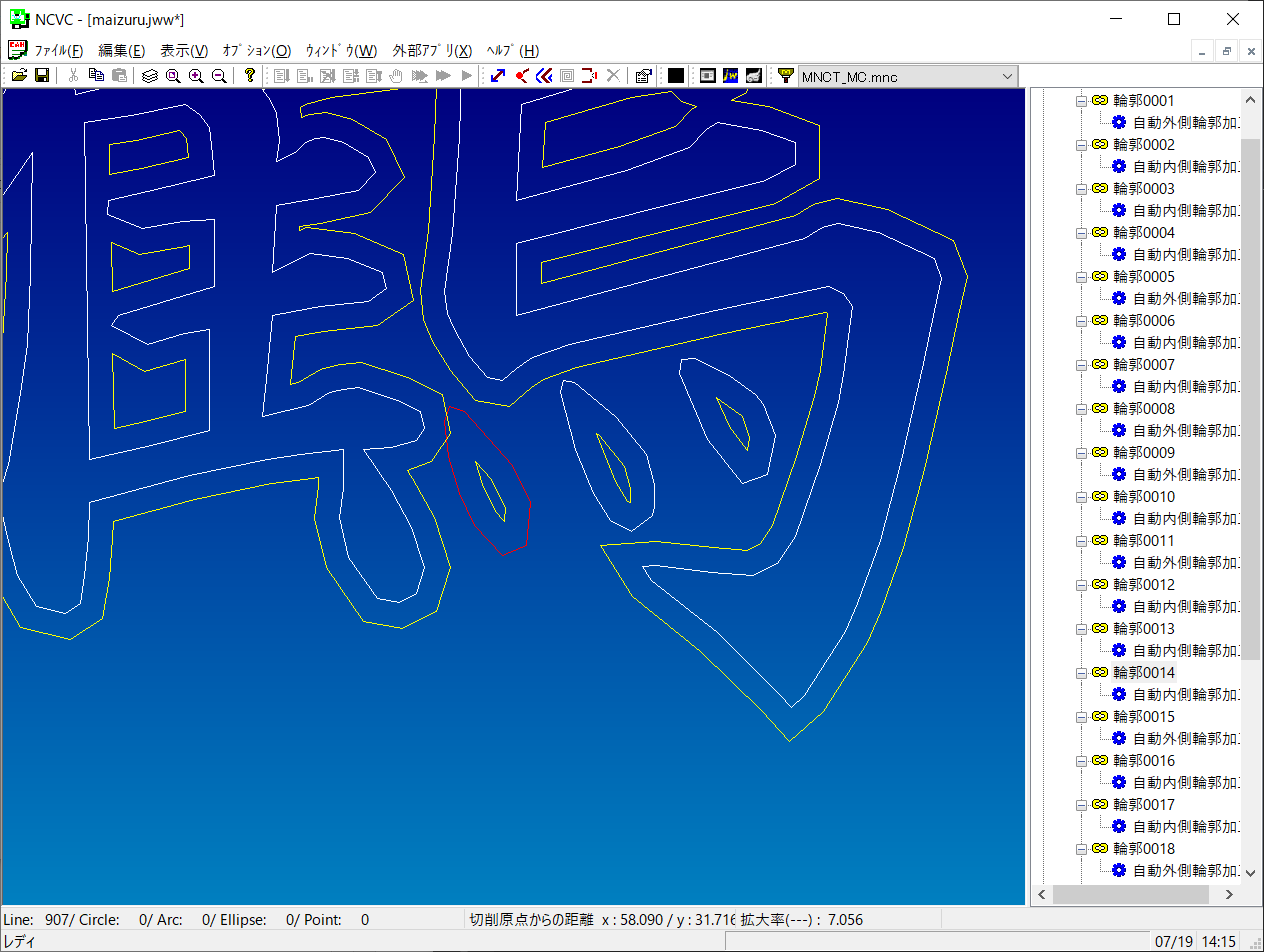
\includegraphics[scale=0.5]{No3/fig/inout1.png}
\caption{オブジェクトの選択}
\label{fig:inout1.png}
\end{figure}

\newpage
%\subsubsection{自動生成の輪郭を削除}
2) \keys{TAB}キーを押すと右側のツリーにフォーカスが移動します.
図形が選択されていると,その図形集合が反転表示されますので,下矢印キーを押し,
輪郭集合が選択された状態で\keys{DEL}キーを押してください.
図\ref{fig:inout2.png} のように輪郭オブジェクトが削除されました.

\begin{figure}[H]
\centering
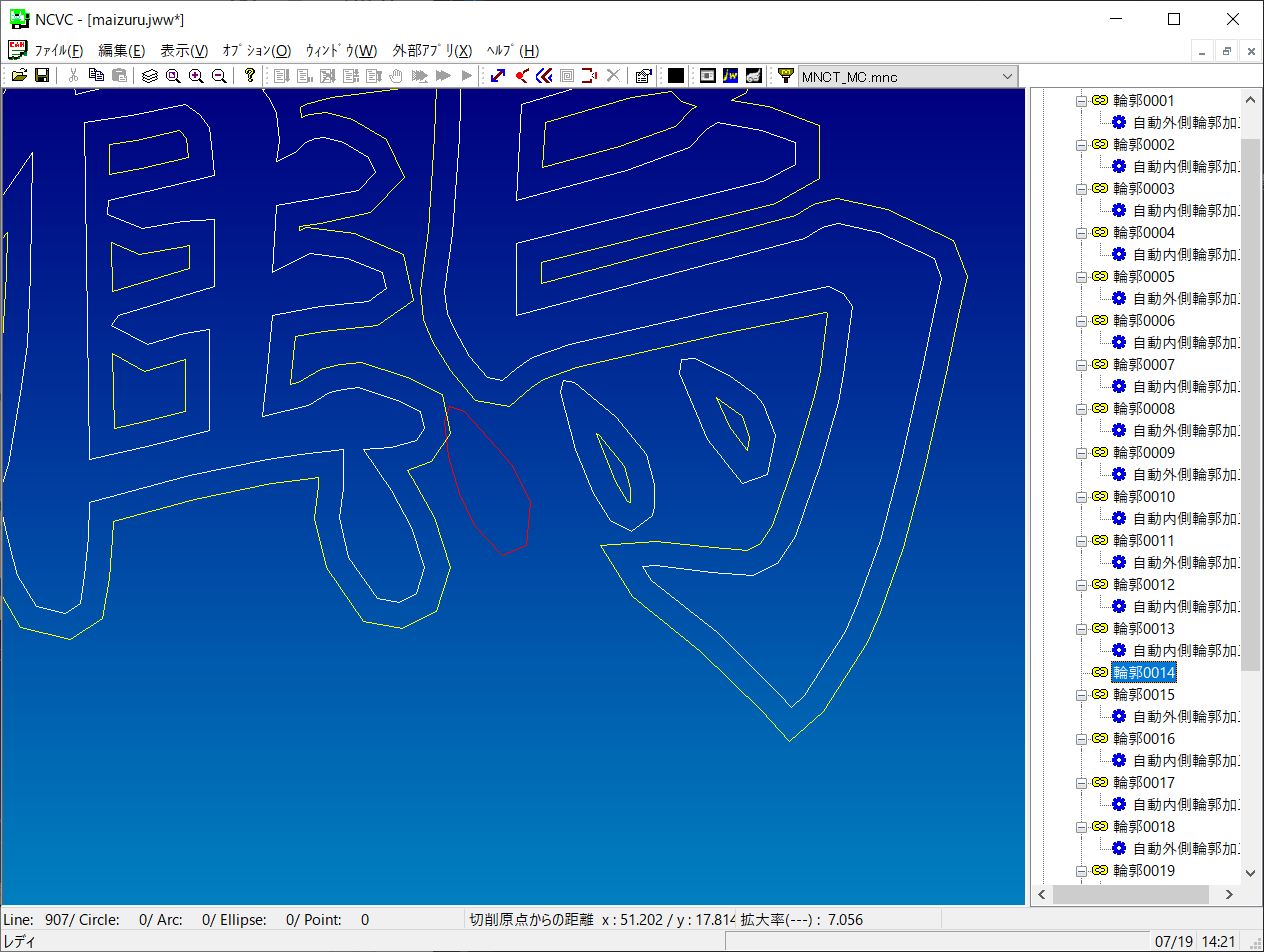
\includegraphics[scale=0.5]{No3/fig/inout2.png}
\caption{自動で生成された輪郭オブジェクトを削除}
\label{fig:inout2.png}
\end{figure}

\newpage
%\subsubsection{手動追加}
3) 加工指示が[輪郭]になっているので,元の図形を(選択された状態で)再クリックすると,一時的な輪郭オブジェクトが生成されます.
マウスを動かし内外の希望する側でクリックしてください.
クリック(決定)すると,図\ref{fig:inout3.png} のように右側のツリーにも該当図形集合に[輪郭加工指示]が追加されます.

\begin{figure}[H]
\centering
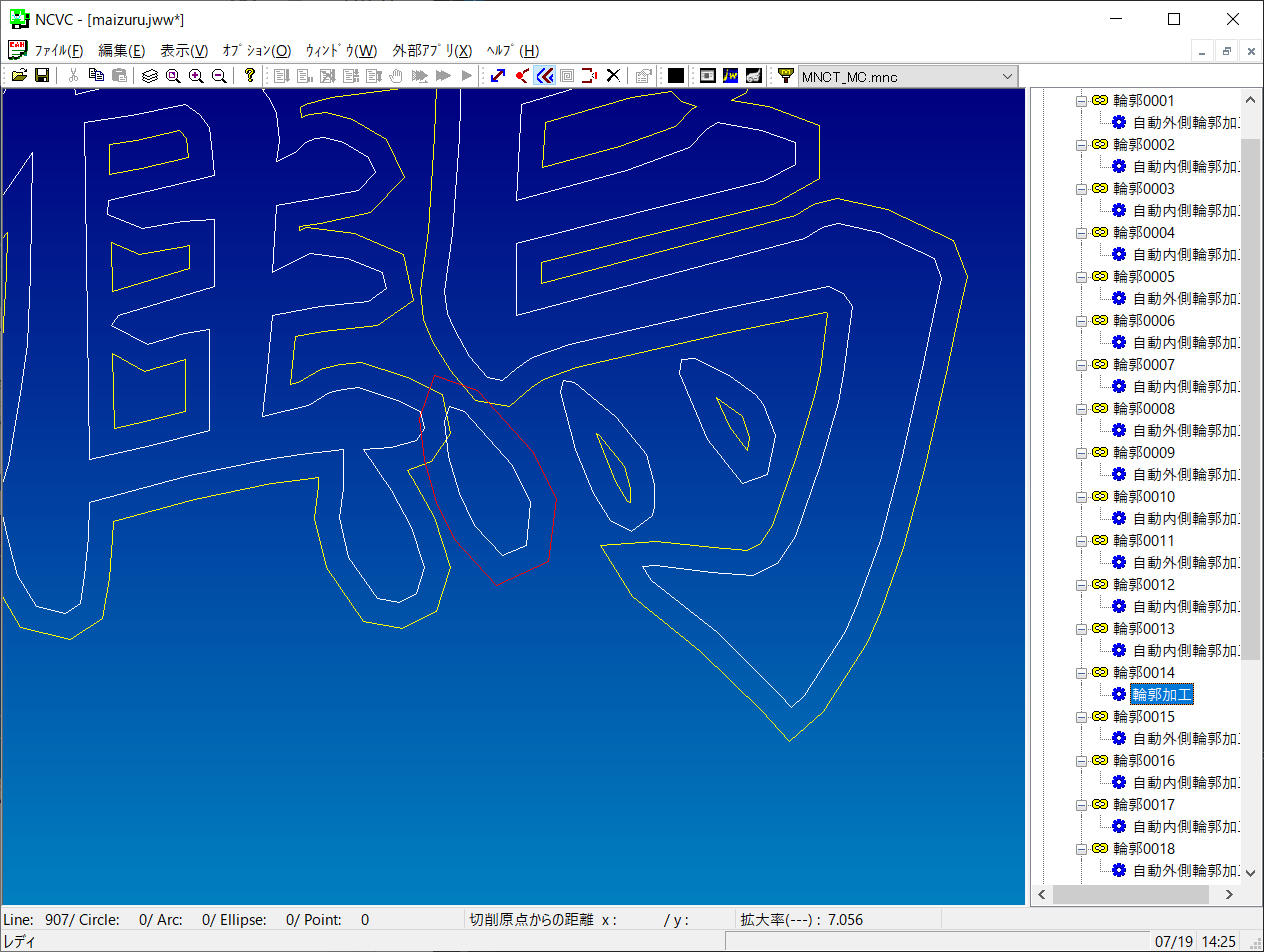
\includegraphics[scale=0.5]{No3/fig/inout3.png}
\caption{手動輪郭設定}
\label{fig:inout3.png}
\end{figure}

\newpage
%\subsubsection{手動調整}
4) 内外の間違っている他の図形集合についても同様に作業を行ってください.
\keys{TAB}キーを有効に使用すると効率よく作業できると思います.
この時点では輪郭同士の交点は気にしなくて結構です.
サンプルでは図\ref{fig:inout4.png} のように設定しました.

\begin{figure}[H]
\centering
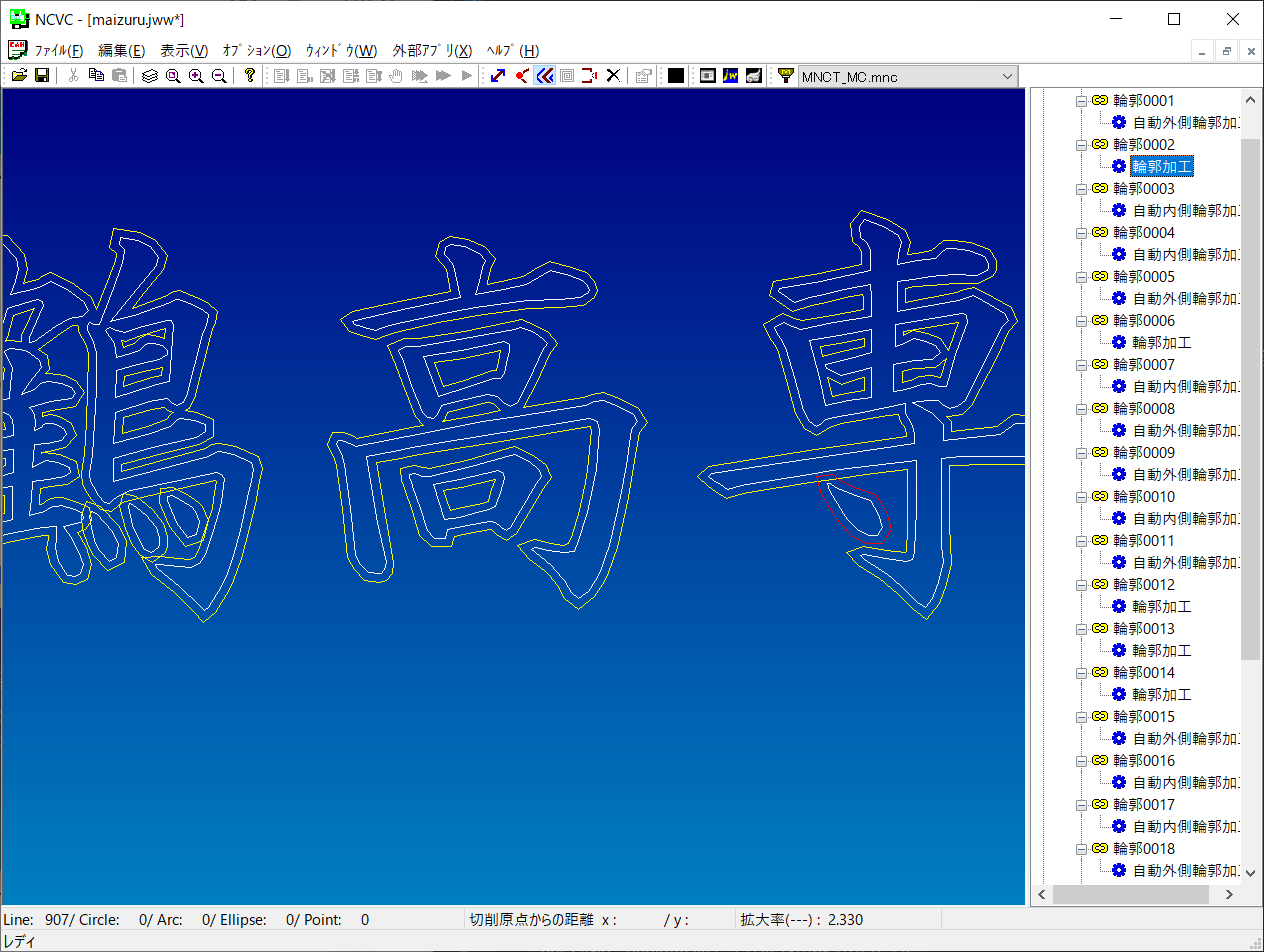
\includegraphics[scale=0.5]{No3/fig/inout4.png}
\caption{手動輪郭による調整完了}
\label{fig:inout4.png}
\end{figure}
